\chapter{状态空间分析方法}
\thispagestyle{empty}
前面几章称为\dy[经典控制理论]{JDKZLL},下面所学的内容称为\dy[现代控制理论]{XDKZLL}。
\begin{table}[!htb]
	\centering
	\setlength{\tabcolsep}{8mm}{
	\begin{tabular}{ccc}
		\toprule
		对比项目 & \makecell[c]{经典控制理论\\(20世纪50年代前)} & \makecell[c]{现代控制理论\\(20世纪50年代后)}\\
		\midrule
		&&\\[-1.5em]
		研究对象 & 单输入单输出的线性定常系统 & 可以比较复杂 \\
		&&\\[-1.5em]
		数学模型 & 传递函数(输入、输出描述)& 状态方程\\
		&&\\[-1.5em]
		数学基础 & 运算微积分、复变函数 & 线性代数、矩阵理论\\
		&&\\[-1.5em]
		设计方法的特点 & \makecell[c]{非唯一性、试凑成分多,经验性强\\主要在复数域进行} & \makecell[c]{设计的解析性,与计算机结合\\主要在时间域进行}\\
		&&\\[-1.5em]
		\bottomrule
	\end{tabular}
}
	\caption{经典控制理论和现代控制理论的简单对比}
\end{table}


\section{状态空间方法基础}
\subsection{状态空间的基本概念}
\vspace*{-1em}
\defination[状态]
动力学系统的\dy[状态]{ZT}可以定义为信息的集合。已知系统$t_0$时的状态、以及$t\ge t_0$的输入,可以确定$t \ge t_0$时系统任一变量的运动状况。
\vspace*{0.5em}

\defination[状态变量]
确定动力学系统状态的一组\textcolor{red}{最小变量}\index{ZTBL@状态变量}:$x_1(t),x_2(t),\cdots x_n(t)$.
\vspace*{0.5em}

\defination[状态向量]
如果完全描述一个给定系统的动态行为需要$n$个状态变量,那么\dy[状态变量]{ZTBL}定义为
\begin{equation}
	\bm{x}(t) \equiv 
	\begin{bmatrix}
		\, x_1(t)\, \\
		\, x_2(t)\, \\
		\, \vdots\, \\
		\, x_n(t)\,
	\end{bmatrix}
\end{equation}

\defination[状态空间]
由状态向量$\bm{x}(t)$张成的$n$维向量空间称为\dy[状态空间]{ZTKJ}。
\vspace*{1em}

\subsection{系统的状态空间表达式}
\noindent \textbf{1. 单输入—单输出线性定常系统}

单输入—单输出线性定常系统
\begin{equation}
	y^{(n)}+a_{n-1}y^{(n-1)} + a_{n-2}y^{(n-2)} + \cdots +a_0 y = u
	\label{单输入输出}
\end{equation}
若给出$t=0$时的初值$y(0), \dot{y}(0), \cdots , y^{n-1}(0)$和$u(t),t \ge 0$时就可以确定系统的行为。

选取状态变量$x_1 = y, x_2 = \dot{y}, \cdots, x_n = y^{(n-1)}$,那么\eqref{单输入输出}可以写为
\begin{equation}
	\begin{aligned}
		\dot{x}_1 &= x_2\\
		\dot{x}_2 &= x_3\\
		&\vdots\\
		\dot{x}_{n-1} &= x_n
	\end{aligned}
	\quad \Rightarrow \quad \dot{x}_n = -a_0x_1-a_1x_2-\cdots -a_{n-1}x_n+u
\end{equation}
方便起见,写出矩阵的形式
\begin{equation}
	\begin{bmatrix}
		 \dot{x}_1\\
		\dot{x}_2\\
		\hspace*{2mm}\vdots\hspace*{2mm}\\
		\dot{x}_{n-1}\\
		\dot{x}_n
	\end{bmatrix}
	=
	\begin{bmatrix}
		0 & 1 & 0 & \cdots & 0\\
		0 & 0 & 1 & \cdots & 0\\
		\vdots & \vdots & \vdots & & \vdots\\
		0 & 0 & 0 & \cdots & 1\\
		-a_0 & -a_1 & -a_2 & \cdots & -a_{n-1}
	\end{bmatrix}
	\,\,
	\begin{bmatrix}
		x_1\\
		x_2\\
		\hspace*{2mm}\vdots\hspace*{2mm}\\
		x_{n-1}\\
		x_{n}
	\end{bmatrix}
	+
	\begin{bmatrix}
		0\\
		0\\
	\hspace*{2mm}\vdots\hspace*{2mm}\\
		0\\
		1
	\end{bmatrix}
	\,\,
	u
\end{equation}
即
\begin{equation}
	\bm{\dot{x}}= \bm{A}\bm{x}+\bm{b}u
\end{equation}

系统的输出为
\begin{equation}
	y = x_1
\end{equation}
同样地,把\dy[输出方程]{SCFC}写出矩阵形式为
\begin{equation}
	y = 
	\begin{bmatrix}
		1&0&\cdots & 0 
	\end{bmatrix}
	\begin{bmatrix}
		x_1\\
		x_2\\
		\hvdots\\
		x_n
	\end{bmatrix} = \bm{c}\bm{x}
\end{equation}

\noindent \textbf{2. 多输入—多输出线性定常系统}

多输入—多输出线性定常系统
\begin{equation}
	\begin{aligned}
		\dot{x}_1 &= a_{11}(t)x_1 + a_{12}(t)x_2 + \cdots + a_{1n}(t)x_n + b_{11}(t)u_1 + \cdots + b_{1p}(t)u_p\\
		\dot{x}_2 &= a_{21}(t)x_1 + a_{22}(t)x_2 + \cdots + a_{2n}(t)x_n + b_{21}(t)u_1 + \cdots + b_{2p}(t)u_p\\
		& \hspace*{12em}\vdots \\
		\dot{x}_n &= a_{n1}(t)x_1 + a_{n2}(t)x_2 + \cdots + a_{nn}(t)x_n + b_{n1}(t)u_1 + \cdots + b_{np}(t)u_p
	\end{aligned}
\end{equation}
写成矩阵形式为
\begin{equation}
	\begin{bmatrix}
		\dot{x}_1\\
		\dot{x}_2\\
		\hspace*{2mm}\vdots\hspace*{2mm}\\
		\dot{x}_n
	\end{bmatrix}
	=
	\begin{bmatrix}
		a_{11} & a_{12}  & \cdots & a_{1n}\\
		a_{21} & a_{22}  & \cdots & a_{2n}\\
		\vdots & \vdots &  & \vdots\\
		a_{n1} & a_{n2}  & \cdots & a_{nn}
	\end{bmatrix}
	\,\,
	\begin{bmatrix}
		x_1\\
		x_2\\
		\hspace*{2mm}\vdots\hspace*{2mm}\\
		x_{n}
	\end{bmatrix}
	+
	\begin{bmatrix}
		b_{11} & b_{12}  & \cdots & b_{1p}\\
		b_{21} & b_{22}  & \cdots & b_{2p}\\
		\vdots & \vdots &  & \vdots\\
		b_{n1} & b_{n2}  & \cdots & b_{np}
	\end{bmatrix}
	\,\,
	\begin{bmatrix}
		{u}_1\\
		{u}_2\\
		\hspace*{2mm}\vdots\hspace*{2mm}\\
		{u}_p
	\end{bmatrix}
\end{equation}
即
\begin{equation}
	\bm{\dot{x}} = \bm{Ax} + \bm{Bu}
\end{equation}

输出方程为
\begin{equation}
	\begin{aligned}
		y_1 &= c_{11}(t)x_1 + c_{12}(t)x_2 + \cdots + c_{1n}(t)x_n + d_{11}(t)u_1 + \cdots + d_{1p}(t)u_p\\
		y_2 &= c_{21}(t)x_1 + c_{22}(t)x_2 + \cdots + c_{2n}(t)x_n + d_{21}(t)u_1 + \cdots + d_{2p}(t)u_p\\
		& \hspace*{12em}\vdots \\
		y_n &= c_{n1}(t)x_1 + c_{n2}(t)x_2 + \cdots + c_{nn}(t)x_n + d_{n1}(t)u_1 + \cdots + d_{np}(t)u_p
	\end{aligned}
\end{equation}
写成矩阵形式为
\begin{equation}
	\begin{bmatrix}
		y_1\\
		y_2\\
		\hspace*{2mm}\vdots\hspace*{2mm}\\
		y_n
	\end{bmatrix}
	=
	\begin{bmatrix}
		c_{11} & c_{12}  & \cdots & c_{1n}\\
		c_{21} & c_{22}  & \cdots & c_{2n}\\
		\vdots & \vdots &  & \vdots\\
		c_{n1} & c_{n2}  & \cdots & c_{nn}
	\end{bmatrix}
	\,\,
	\begin{bmatrix}
		x_1\\
		x_2\\
		\hspace*{2mm}\vdots\hspace*{2mm}\\
		x_{n}
	\end{bmatrix}
	+
	\begin{bmatrix}
		d_{11} & d_{12}  & \cdots & d_{1p}\\
		d_{21} & d_{22}  & \cdots & d_{2p}\\
		\vdots & \vdots &  & \vdots\\
		d_{n1} & d_{n2}  & \cdots & d_{np}
	\end{bmatrix}
	\,\,
	\begin{bmatrix}
		{u}_1\\
		{u}_2\\
		\hspace*{2mm}\vdots\hspace*{2mm}\\
		{u}_p
	\end{bmatrix}
\end{equation}
即
\begin{equation}
	\bm{y} = \bm{Cx} + \bm{Du}
\end{equation}

\vspace*{1em}

\subsection{线性定常系统状态方程的解}
\noindent \textbf{1. 齐次状态方程的解}

齐次向量微分方程
\begin{equation}
	\dot{\bm{x}}=\bm{Ax}
\end{equation}
方程的解为
\begin{equation}
	\bm{x}(t) = \bm{b}_0+\bm{b}_1t + \bm{b}_2t^2 + \cdots + \bm{b}_kt^k + \cdots
	\label{齐次向量微分方程}
\end{equation}
其中,$\bm{b}_i$为列向量。将$\bm{x}(t)$代入方程$\dot{\bm{x}}=\bm{Ax}$,可得
\begin{equation}
	\bm{b}_1 + 2\bm{b}_2t + \cdots + h\bm{b}_kt^{k-1} + \cdots = \bm{A}\big(\bm{b}_0 + \bm{b}_1 + \cdots + \bm{b}_kt^k + \cdots\big)
\end{equation}
方程两边系数必相等,即
\begin{equation}
	\begin{cases}
		\, \bm{b}_1 = \bm{Ab}_0\\[0.5em]
		\, \bm{b}_2 = \dfrac{1}{2}\bm{Ab}_1=\dfrac{1}{2}\bm{A}^2\bm{b}_0\\[0.5em]
		\, \bm{b}_3 = \dfrac{1}{3}\bm{Ab}_2 = \dfrac{1}{3\times 2}\bm{A}^3\bm{b}_0\\[0.5em]
		\, \hspace*{3em}\vdots\\[0.5em]
		\, \bm{b}_k = \dfrac{1}{k!}\bm{A}^k\bm{b}_0\\[0.5em]
	\end{cases}
\end{equation}
将$t=0$代入公式\eqref{齐次向量微分方程},可以得到
\begin{equation}
	\bm{b}_0 = \bm{x}(0) \triangleq \bm{x}_0
\end{equation}
所以齐次状态方程的解为
\begin{equation}
	\bm{x}(t) = \left(\bm{I} + \bm{A}t + \dfrac{1}{2!}\bm{A}^2t^2 + \cdots + \dfrac{1}{k!}\bm{A}^kt^k+ \cdots\right)\bm{x}_0
\end{equation}
定义
\begin{equation}
	\e^{\bm{A}t} = \bm{I} + \bm{A}t + \dfrac{1}{2!}\bm{A}^2t^2 + \cdots + \dfrac{1}{k!}\bm{A}^kt^k+ \cdots
\end{equation}
为\dy[矩阵指数]{JZZS},其为$n \times n$矩阵。于是齐次方程的解为
\begin{equation}
	\bm{x}(t) = \e^{\bm{A}t}\bm{x}(0)
\end{equation}
记$\bm{\varPhi(t)}=\e^{\bm{A}t}$,称为\dy[状态转移矩阵]{ZTZYJZ}。关于$\bm{\varPhi}(t)$,有如下的定理

\theorem[状态转移矩阵的性质]
$\bm{\varPhi(t)}$是矩阵微分方程
\begin{equation}
	\begin{cases}
		\, \dot{\bm{\varPhi}}(t) = \bm{A}\bm{\varPhi}(t)\\
		\, \bm{\varPhi}(0) = \bm{I}
	\end{cases}
\end{equation}
的唯一解。同时,状态转移方程还具有如下的性质
\begin{enumerate}[\hspace*{2em} \textbf{性质} 1]
	\item 
	\begin{equation}
		\bm{\varPhi}(0) = \bm{I}
	\end{equation}
	\item 
	\begin{equation}
		\bm{\varPhi}^{-1}(t) = \bm{\varPhi}(-t)
	\end{equation}

	\item 
	\begin{equation}
		\bm{\varPhi}(t_2 - t_1)\bm{\varPhi}(t_1 - t_0) = \bm{\varPhi}(t_2 - t_0)
	\end{equation}
	根据转移矩阵的这个性质,可以把一个转移过程分成若干个小的转移过程来研究。
	
	\item 
	\begin{equation}
		\big[\bm{\varPhi(t)}\big]^k = \bm{\varPhi}(kt)
	\end{equation}
\end{enumerate}
\vspace*{0.5em}

\noindent \textbf{2. $\e^{\bm{A}t}$的求解}
\begin{enumerate}[\hspace*{1em} (1) ]
	\item \textbf{利用无穷级数}
	
	\defination[矩阵函数的幂级数]
	 设函数$f(\lambda)$的幂级数表示为
	 \begin{equation}
	 	f(\lambda) = \sum_{i = 0}^{\infty} \alpha_i \lambda^i
	 \end{equation}
	其收敛半径为$\rho$,如果$\bm{A}$的所有特征值的绝对值小于$\rho$,或者对于某个正整数$k$,有$\bm{A}^k = 0$,则
	
	有了矩阵函数的幂级数的定义,利用$\e^{\bm{A}t}$的无穷级数展开,得
	\begin{equation}
		\e^{\bm{A}t} = \bm{I} + \bm{A}t + \dfrac{\bm{A}^2}{2!}t^2 + \dfrac{\bm{A}^3}{3!}t^3 + \cdots = \sum_{k=0}^{\infty} \dfrac{\bm{A}^k}{k!}t^k
	\end{equation}

	\item \textbf{利用方阵函数计算$\e^{\bm{A}t}$}
	
	\defination[矩阵函数的多项式]
	\hspace*{2em} 设$f(\lambda)$是定义在$\bm{A}$的频谱上的函数,若$g(\lambda)$是多项式且在$\bm{A}$的频谱上与$f(\lambda)$具有相同的值,则矩阵值函数$f(\bm{A})$定义为$f(\bm{A}) \triangleq g(\bm{A})$.
	
	设$\bm{A}$的特征多项式为
	\begin{equation}
		\Delta (\lambda) \triangleq \det\big(\lambda \bm{I} - \bm{A}\big) = \prod_{i=1}^{m}\big(\lambda - \lambda_i\big)^{n_i}\quad \left(\sum_{i = 1}^{m}n_i = n\right)
	\end{equation}
	令$f,g$是两个任一的多项式,若满足$f^{(l)}(\lambda_i)= g^{(l)}(\lambda_i)\,\,(i=1,2,\cdots,m;\, l=0,1,\cdots, n_i-1)$,则$f(\bm{A}) = g(\bm{A})$.
	
	所有$f^{(l)}(\lambda_i)\,\,(i=1,2,\cdots,m;\, l=0,1,\cdots, n_i-1)$(共有$\displaystyle \sum_{i=1}^{m}n_i$个)的集合称为$f$在$\bm{A}$的频谱上的值。根据矩阵函数多项式的定义,如果$\bm{A}$是$n \times n$矩阵,给定了$f(\lambda)$在$\bm{A}$的频谱上的$n$个值,就能找到$n-1$次多项式
	\begin{equation}
		g(\lambda) = \alpha_0 + \alpha_1\lambda + \cdots + \alpha_{n-1}\bm{A}^{n-1}
	\end{equation}
	它在$\bm{A}$的频谱上与$f(\lambda)$相等,则
	\begin{equation}
		f(\bm{A}) = \alpha_0 \bm{I} + \alpha_1 \bm{A} + \cdots + \alpha_{n-1}\bm{A}^{n-1}
	\end{equation}

	\item \textbf{利用$\e^{\bm{A}t} = \mathcal{L}^{-1}\big[(s\bm{I} - \bm{A})^{-1}\big]$}\\
	\hspace*{1em} 先求$s\bm{I} - \bm{A}$的逆变换,再求Laplace逆变换,这个方法最常用。逆变换的求法有:
	\begin{itemize}
		\item 代数余子式
		\begin{equation}
			\bm{A}^{-1} = \dfrac{1}{\det \bm{A}}\text{adj}(\bm{A})
		\end{equation}
		\item 增广矩阵$+$矩阵初等变换
		\begin{equation}
			\bm{AE} \sim \bm{EA^{-1}}
		\end{equation}
	\end{itemize}
\end{enumerate}
\vspace*{0.5em}

\noindent \textbf{3. 非其次方程的解}

非齐次方程
\begin{equation}
	\bm{\dot{x}}(t) = \bm{Ax}(t) + \bm{Bu}(t)
\end{equation}
改写为
\begin{equation}
	\bm{\dot{x}}(t) - \bm{Ax}(t) = \bm{Bu}(t)
\end{equation}
用$\e^{-\bm{A}t}$左乘等式两边,得
\begin{equation}
	\e^{-At}[\dot{\bm{x}}(t) - \bm{Ax}(t)] = \dfrac{\d }{\d t}\big[\e^{-\bm{A}t} \bm{x}(t)\big] = \e^{-\bm{A}t}\bm{Bu}(t)
\end{equation}
积分可得
\begin{equation}
	\e^{-\bm{A}t}\bm{x}(t) = \bm{x}_0 + \int_0^t \e^{-\bm{A}\tau}\bm{Bu(\tau)}\, \d \tau
\end{equation}
用$\e^{\bm{A}t}$左乘等式两边,得
\begin{equation}
	\bm{x}(t) = \e^{\bm{A}t}\bm{x}(0) + + \int_0^t \e^{-\bm{A}(t - \tau)}\bm{Bu(\tau)}\, \d \tau
\end{equation}
即
\begin{equation}
	\bm{x}(t) = \bm{\varPhi}(t)\bm{x}(t) + \int_0^t \bm{\varPhi}(t - \tau)\bm{Bu}(\tau)\, \d \tau
\end{equation}

\subsection{传递函数矩阵}
系统的状态方程和输出方程为
\begin{align*}
	\dot{\bm{x}}&=\bm{Ax} + \bm{Bu}\\
	\bm{y} &= \bm{Cx} + \bm{Du}
\end{align*}
零初始条件下的Laplace变换为
\begin{align*}
	s\bm{x}(s) &= \bm{Ax}(s) + \bm{Bu}(s)\\
	\bm{y}(s) & = \bm{Cx}(s) + \bm{Du}(s)
\end{align*}
解得
\begin{align}
	\bm{x}(s) &= (s\bm{I}- \bm{A})^{-1}\bm{Bu}(s)\\
	\bm{y}(s) &= \big[\bm{C}(s\bm{I} - \bm{A})^{-1}\bm{B} + \bm{D}\big]\bm{u}(s)
\end{align}

定义\dy[传递函数矩阵]{CDHSJZ}为
\begin{equation}
	\bm{G}(s) = \bm{C}(s\bm{I} - \bm{A})^{-1}\bm{B} + \bm{D}
\end{equation}
由逆矩阵的计算,可以得到
\begin{equation}
	\bm{G}(s) = \bm{C}\dfrac{\text{adj}(s\bm{I}-\bm{A})}{\det (s \bm{I} - \bm{A})}\bm{B} + \bm{D}
	= \bm{C}\dfrac{\text{adj}(s\bm{I}-\bm{A}) + (s\bm{I}-\bm{A})\bm{D}}{\det (s \bm{I} - \bm{A})}
\end{equation}
可以得到其特征方程为
\begin{equation}
	\det (s \bm{I} - A) = 0
\end{equation}

\subsection{动态方程的可逆线性变化}



\section{线性系统的可控性和可观性}
状态空间法,对系统的表述如下:
\begin{equation*}
	\mbox{系统}\,
	\begin{cases}
		\, \mbox{状态方程} \xrightarrow{\quad}\mbox{由输入和初始状态所引起的状态变化}\xrightarrow{\mbox{\small \quad 输入是否能控制状态变化 \quad }}\mbox{\dy[可控性]{KKX}}\\[1em]
		\, \mbox{输出方程} \xrightarrow{\quad}\mbox{由状态变化而引起输出的变化}\xrightarrow{\mbox{\small \quad 输出是否能反映状态变化 \quad }}\mbox{\dy[可观测性]{KGCX}}
	\end{cases}
\end{equation*}

\subsection{准备知识}
\noindent \textbf{1. 齐次方程组的非零解}

设$\bm{A}$是$n\times n$矩阵,$\bm{x}$是$n \times 1$向量,齐次方程组
\begin{equation}
	\bm{Ax} = \bm{0}
	\label{齐次方程组}
\end{equation}
$|\bm{A}| = 0 \xrightarrow{\quad \quad }$方程\eqref{齐次方程组}存在非零解,$|\bm{A}| \neq 0 \xrightarrow{\quad \quad }$方程\eqref{齐次方程组}只有零解。
\vspace*{1em}

\noindent \textbf{2. 凯莱—哈米尔顿定理\index{KLHEMD@凯莱—哈米尔顿定理}}

\dy[Cayley-Hamilton定理]{CAYLEY}说明了:\textbf{矩阵$\bm{A}$满足自己的特征多项式},即

若$\bm{A}$的特征多项式为
\begin{equation}
	f(\lambda) = |\lambda \bm{I} - \bm{A}| = \lambda^n + a_{n-1}\lambda^{n-1} + \cdots + a_1 \lambda + a_0
\end{equation}
则$\bm{A}$满足
\begin{equation}
	f(\bm{A}) = \bm{A}^n + a_{n-1}\bm{A}^{n-1} + \cdots + a_1 \bm{A}+ a_0 \bm{I} = 0
\end{equation}

应用Cayley-Hamilton定理,可得
\begin{equation}
	\bm{A}^n = - \big(a_{n-1}\bm{A}^{n-1} + \cdots + a_1 \bm{A} + a_0 \bm{I}\big)
\end{equation}
也就是说,对于矩阵指数$\e^{\bm{A}t}$,$\bm{A}^k(k \ge n)$可以用$\bm{A}^{n-1}, \bm{A}^{n-2}, \cdots, \bm{A}, \bm{A}^0 = \bm{I}$来表示,即
\begin{equation}
	\e^{\bm{A}t} = \sum_{k = 0}^{n - 1}\alpha_k(t)\bm{A}^k
\end{equation}
\vspace*{0.5em}

\noindent \textbf{3. 引理}
\begin{equation}
	\text{rank}
	\begin{bmatrix}
		\bm{b} & \bm{Ab} & \bm{A}^2\bm{b} &\cdots & \bm{A}^{n-1}\bm{b}
	\end{bmatrix}
	= n
\end{equation}
的充要条件是:存在$t_1 > 0$使得
\begin{equation}
	\bm{W}(0,t_1) = \int_0^{t_1}\e^{-\bm{A}t}\bm{b}\bm{b}^{\text{T}}\e^{-\bm{A}^{\text{T}}t}\, \d t
\end{equation}
非奇异。这里$\bm{A}$是$n \times n$矩阵,$\bm{b}$是$n \times 1$向量。
\vspace*{1em}

\subsection{线性系统的可控性}
\noindent \textbf{1. 可控性的定义}

如图\ref{状态转移},对于任意时刻$t_0$和$t_f$,若存在控制向量$\bm{u}(t)$,能将$t = t_0$的每个初始状态$\bm{x}(t_0)$转移到$t = t_f$时刻的另一任意状态$\bm{x}(t_f)$,则称此系统的状态完全可控。

\begin{figure}[!htb]
	\centering
	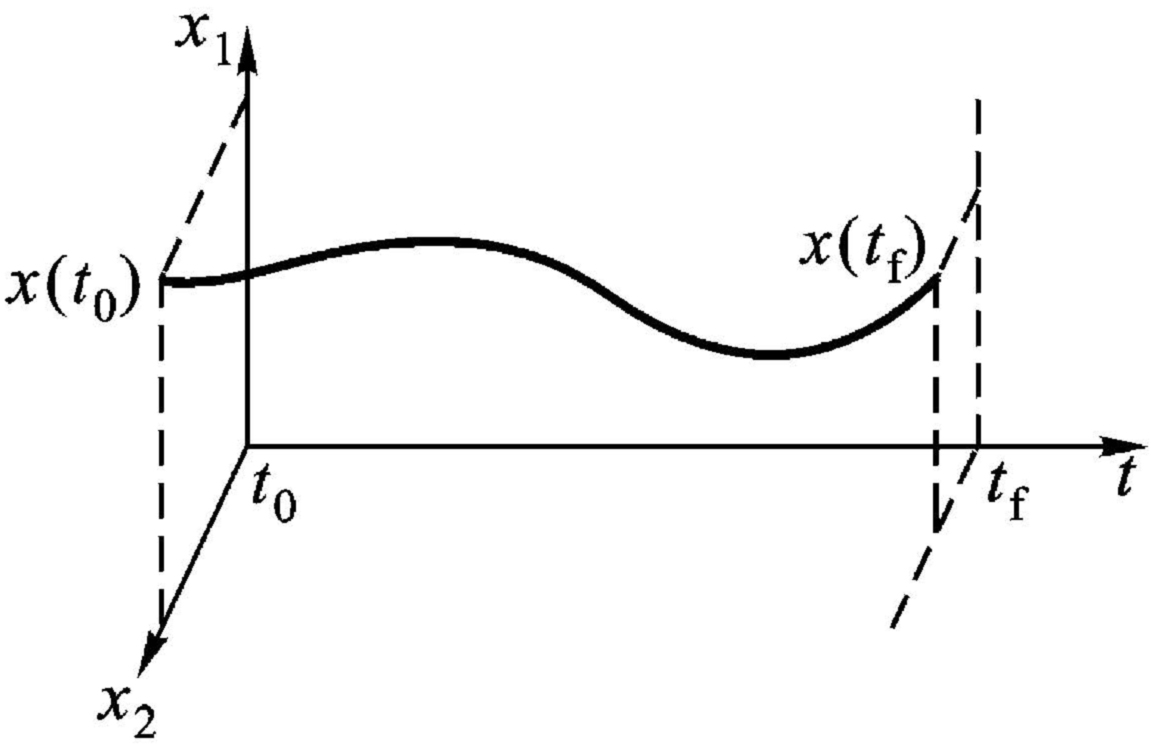
\includegraphics[width=0.3\linewidth]{pic/状态转移.jpg}
	\caption{状态转移过程}
	\label{状态转移}
\end{figure}

\noindent \textbf{2. 可控性判据}

单变量线定常系统
\begin{align}
	\dot{\bm{x}} &= \bm{Ax} + \bm{b}u\\
	y &= \bm{cx} + du 
\end{align}
其中,$\bm{A}:(n\times n),\bm{b}:(n\times 1), \bm{c}:(1\times n), d(1\times 1)$。则系统可控的充分必要条件为
\begin{equation}
	\text{rank}
	\begin{bmatrix}
		\bm{b} & \bm{Ab} & \cdots & \bm{A}^{n-1}\bm{b}
	\end{bmatrix} = n
\end{equation}
将上述矩阵记为\dy[可控性矩阵]{KKXJZ}
\begin{equation}
	\bm{S} = 
	\begin{bmatrix}
		\bm{b} & \bm{Ab} & \cdots & \bm{A}^{n-1}\bm{b}
	\end{bmatrix} = n
\end{equation}
可控的充要条件就写为
\begin{equation}
	\text{rank}\,\bm{S} = n \quad \Longleftrightarrow \quad \det \bm{S} \neq 0
\end{equation}
\vspace*{0.5em}

\noindent \textbf{3. 约当型方程的可控性判据}

由于矩阵的等价变换不影响系统的可控性,约当块的一般形式为
\begin{equation}
	\bm{\varLambda}_1 =
	\begin{bmatrix}
		\lambda_1 & 1 & 0 & \cdots & 0 \\
		& \lambda_1 & 1 & & 0\\
		& & \ddots & \ddots &\vdots \\
		& & & \lambda_1 & 1\\
		& & & & \lambda_1
	\end{bmatrix}
\end{equation}
若系数矩阵$\bm{A}$满足具有约当块的形式,可控的充分必要条件为
\begin{enumerate}[\hspace*{2em} (1)]
	\item 同一特征值对应的约当块只有一块,即各约当块的特征值不同。
	\item 每一约当块最后一行,所对应的$b$中的元素不为零。
\end{enumerate}
这一充分必要条件又称为\textbf{单输入系统约当形方程的可控性判据}。

\examples 已知系统的状态方程为
\begin{equation*}
	\dot{\bm{x}} =
	\begin{bmatrix}
		\lambda_1 & 1 & &\\
		& \lambda_1 & & \\
		& & \lambda_2 & 1 \\
		& &  & \lambda_1 
	\end{bmatrix}
	\bm{x} +
	\begin{bmatrix}
	\hspace*{1mm}	b_1 \hspace*{1mm}\\
		b_2\\
		b_3\\
		b_4
	\end{bmatrix}
	\bm{u}
\end{equation*}
确定系统可控时,$\lambda_1, \lambda_2, b_i$应满足的条件。

\solve 矩阵$\bm{A}$具有约当块的形式,可以分为两个约当块
\begin{equation*}
	\bm{\varLambda}_1 = 
	\begin{bmatrix}
		\lambda_1 & 1\\
		& \lambda_1
	\end{bmatrix},
	\bm{B}_1 = 
	\begin{bmatrix}
		\hspace*{1mm}	b_1 \hspace*{1mm}\\
		b_2\\
	\end{bmatrix}\quad 
	\bm{\varLambda}_2 =
	\begin{bmatrix}
		\lambda_2 & 1\\
		& \lambda_2
	\end{bmatrix},	
	\bm{B}_2 = 
	\begin{bmatrix}
	\hspace*{1mm}	b_3 \hspace*{1mm}\\
	b_4\\
	\end{bmatrix}
\end{equation*}
	由单输入系统约当形方程的可控性判据,可知
	\begin{enumerate}[\hspace*{2em} (1)]
		\item $\lambda_1 \neq \lambda_2$(各个约当块)
		\item $b_2,b_4 \neq 0$
	\end{enumerate}
	综合以上条件,系统可控的充要条件为
	\begin{equation*}
		(\lambda_1 - \lambda_2 )b_2b_4 \neq 0
	\end{equation*}
\vspace*{0.5em}

\noindent \textbf{4. 可控标准形}

一个单输入系统,如果具有如下形式
\begin{equation}
	\dot{\bm{x}} = 
	\begin{bmatrix}
		0 & 1 & 0 & 0 & 0 \\
		0 &   & 1 &   & 0\\
		\vdots & \vdots & \vdots & \ddots & \vdots\\
		0 & 0 & 0 & 0 & 1\\
		-\alpha_0 & -\alpha_1 & -\alpha_2 & \cdots & - \alpha_{n-1} 
	\end{bmatrix}
	\bm{x} +
	\begin{bmatrix}
		0\\
		0\\
		\vdots\\
		0\\
		1
	\end{bmatrix}
	u
	\label{标准形}
\end{equation}
则系统一定可控,公式\eqref{标准形}的形式被称为单输入系统的\dy[可控标准形]{KKBZX}。
\vspace*{1em}

\noindent \textbf{5. 可控系统方程转换为标准形式}	

对于一般的单输入$n$维动态方程
\begin{equation}
	\dot{\bm{x}} = \bm{Ax} + \bm{b}u
\end{equation}
其中,$\bm{A}:(n \times n), \bm{b}: (n \times 1)$的矩阵。则满足:

若$n$维单输入系统可控,则存在可逆线性变换,将其变换成可控标准形。
\vspace*{0.5em}

\example[可控系统方程转换为标准形式]
\vspace*{-1.5em}
\begin{enumerate}[\textbf{步骤} 1 ]
	\item \textbf{计算可控性矩阵并判断系统的可控性}
	\begin{equation}
		\bm{S} = 
		\begin{bmatrix}
			\bm{b} & \bm{Ab} & \cdots & \bm{A}^{n-1}\bm{b}
		\end{bmatrix} 
	\end{equation}
	\item \textbf{计算$\bm{S}^{-1}$,并记$\bm{S}^{-1}$的最后一行为$\bm{h}$}
	\item \textbf{构造矩阵$\bm{P}$}
	\begin{equation}
		\bm{P} = 
		\begin{bmatrix}
			\bm{h}\\
			\bm{hA}\\
			\bm{hA}^2\\
			\vdots\\
			\bm{hA}^{n-1}
		\end{bmatrix}
	\end{equation}
	\item \textbf{作线性变换}
	\begin{align}
		\overline{\bm{x}} & = \bm{Px}\\
		\overline{\bm{A}} & = \bm{PAP}^{-1}\\
		\overline{\bm{B}} & = \bm{PB}\\
		\overline{\bm{C}} & = \bm{CP}^{-1}\\
		\overline{\bm{D}} & = \bm{D}
	\end{align}
\end{enumerate}

\examples 设系统的状态方程为
\begin{equation*}
	\dot{\bm{x}} = 
	\begin{bmatrix}
		-2 & 2 & -1\\
		0 & -2 & 0\\
		1 & -4 & 0
	\end{bmatrix}
	\bm{x} +
	\begin{bmatrix}
		\hspace*{0.5mm}0\hspace*{0.5mm}\\
		1\\
		1
	\end{bmatrix}
	u
\end{equation*}
将系统状态方程化为可控标准形。

\solve 按照解题方法解题。
\begin{enumerate}[\textbf{步骤} 1 ]
	\item \textbf{计算可控性矩阵并判断系统的可控性}
	\begin{equation*}
		\bm{S} = 
		\begin{bmatrix}
			\bm{b} & \bm{Ab} & \cdots & \bm{A}^{n-1}\bm{b}
		\end{bmatrix} = 
		\begin{bmatrix}
			0 & 1 & -2\\
			1 & -2 & 4\\
			1 & -4 & 9
		\end{bmatrix}
		\qquad \det S \neq 0
	\end{equation*}
	\item \textbf{计算$\bm{S}^{-1}$,并记$\bm{S}^{-1}$的最后一行为$\bm{h}$}
	\begin{equation*}
		\bm{S}^{-1} = 
		\begin{bmatrix}
			2 & 1 & 0\\
			5 & -2 & 2\\
			2 & -1 & 1
		\end{bmatrix}
	\qquad \bm{h} = 
	\begin{bmatrix}
		2 & -1 & 1
	\end{bmatrix}
	\end{equation*}

	\item \textbf{构造矩阵$\bm{P}$}
	\begin{equation}
		\bm{P} = 
		\begin{bmatrix}
			\bm{h}\\
			\bm{hA}\\
			\bm{hA}^2\\
			\cdots\\
			\bm{hA}^{n-1}
		\end{bmatrix}
	= 
	\begin{bmatrix}
		2 & -1 & 1\\
		-3 & 2 & -2\\
		4 & -2 & 3
	\end{bmatrix}
	\qquad \bm{P}^{-1} =
	\begin{bmatrix}
		2 & 1 & 0\\
		1 & 2 & 1\\
		-2 & 0 & 1
	\end{bmatrix}
	\end{equation}
	\item \textbf{作线性变换}
	\begin{align*}
		\overline{\bm{A}} & = \bm{PAP}^{-1} =
		\begin{bmatrix}
			2 & -1 & 1\\
			-3 & 2 & -2\\
			4 & -2 & 3
		\end{bmatrix}
		\begin{bmatrix}
			-2 & 2 & -1\\
			0 & -2 & 0\\
			1 & -4 & 0
		\end{bmatrix}
		\begin{bmatrix}
			2 & 1 & 0\\
			1 & 2 & 1\\
			-2 & 0 & 1
		\end{bmatrix}
		= 
		\begin{bmatrix}
			0 & 1 & 0\\
			0 & 0 & 1\\
			-2 & -5 & -4
		\end{bmatrix}
		\\[1em]
		\overline{\bm{B}} & = \bm{PB} = 
		\begin{bmatrix}
			2 & -1 & 1\\
			-3 & 2 & -2\\
			4 & -2 & 3
		\end{bmatrix}
		\begin{bmatrix}
			\hspace*{0.5mm}0\hspace*{0.5mm}\\
			1\\
			1
		\end{bmatrix}
		= 
		\begin{bmatrix}
			\hspace*{0.5mm}0\hspace*{0.5mm}\\
			0\\
			1
		\end{bmatrix}
		\\
	\end{align*}
\end{enumerate}

\noindent \textbf{6. 系统按可控性分解}

系统不完全可控时,有
\begin{equation}
	\text{rank}
	\begin{bmatrix}
		\bm{b} & \bm{Ab} & \cdots & \bm{A}^{n-1}\bm{b}
	\end{bmatrix}
	= n_1 < n
	\label{不可控}
\end{equation}
这时,有\textbf{系统按可控性进行分解的定理}:

若单变量系统的可控性矩阵满足公式\eqref{不可控},则存在可逆线性变换矩阵$\bm{P}$,使得变换后的系统方程具有以下形式:
\begin{align}
	\begin{bmatrix}
		\hspace*{0.5mm}\dot{\overline{\bm{x}}}_1 \hspace*{0.5mm}\\
		\dot{\overline{\bm{x}}}_2 \\
	\end{bmatrix}
	&=
	\begin{bmatrix}
		\bm{A}_1 & \bm{A}_2\\
		0 & \bm{A}_4
	\end{bmatrix}
	\begin{bmatrix}
		\hspace*{0.5mm}\overline{\bm{x}}_1 \hspace*{0.5mm}\\
		\overline{\bm{x}}_2 \\
	\end{bmatrix}
	+
	\begin{bmatrix}
	\hspace*{0.5mm}	\bm{b}_1 \hspace*{0.5mm}\\
		0
	\end{bmatrix}u \\[1em]
	y &= 
	\begin{bmatrix}
		\bm{c}_1 & \bm{c}_2 
	\end{bmatrix}
	\begin{bmatrix}
		\hspace*{0.5mm}\overline{\bm{x}}_1 \hspace*{0.5mm}\\
		\overline{\bm{x}}_2 \\
	\end{bmatrix}
	+ du
	\label{传递函数不变}
\end{align}
其中,$\overline{\bm{x}}_1:(1 \times n_1),\overline{\bm{x}}_2:(1 \times n_2)$,且
\begin{align}
	\text{rank} = 
	\begin{bmatrix}
		\bm{b}_1 & \bm{A}_1\bm{b}_1 & \cdots & \bm{A}_1^{n_1-1}\bm{b}_1
	\end{bmatrix}
	= n_1\\[0.5em]
	\bm{c}\big(s\bm{I}-\bm{A}\big)^{-1}\bm{b} + d = \bm{c}_1 \big(\bm{I}_{n_1} - \bm{A}_1\big)^{-1}\bm{b}_1 + d
\end{align}
所以,以下的动态方程是可控的
\begin{align}
	\dot{\overline{\bm{x}}}_1 &= \bm{A}_1 \overline{\bm{x}}_1 + \bm{b}_1 u\\
	y_1 & = \bm{c}_1 \overline{\bm{x}}_1 + du
\end{align}

由公式\eqref{传递函数不变}说明分解前后的系统状态方程具有相同的传递函数。或者说\textcolor{red}{传递函数中未能反映系统中不可控的部分}。

\vspace*{0.5em}

\example[系统的可控性分解]
\vspace*{-1em}
\begin{enumerate}[\textbf{步骤} 1 ]
	\item \textbf{计算可控性矩阵并判断系统的可控性}
	\begin{equation}
		\text{rank}\, \bm{S} = \text{rank}\,
		\begin{bmatrix}
			\bm{b} & \bm{Ab} & \cdots & \bm{A}^{n-1}\bm{b}
		\end{bmatrix} = n_1 < n
	\end{equation}
	\item \textbf{从左至右依次搜索$\bm{S}$的线性无关列,直到找到某列线性相关于它左方各列},即
	\begin{equation}
		\text{rank} 
		\begin{bmatrix}
			\bm{b} &  \bm{Ab} & \cdots & \bm{A}^{n_1-1}\bm{b}
		\end{bmatrix}
	 = n_1
	\end{equation}
	
	\item \textbf{补充选取线性无关的向量}
	\begin{equation}
		\begin{bmatrix}
		 \bm{q}_{n_1+1} & \bm{q_{n_1+2}} & \cdots & \bm{q}_n
		\end{bmatrix}
	\end{equation}
	并使得向量组
	\begin{equation}
		\begin{bmatrix}
			\bm{b} & \bm{Ab} & \cdots & \bm{A}^{n_1 - 1}\bm{b} & \bm{q}_{n_1+1} & \bm{q_{n_1+2}} & \cdots & \bm{q}_n
		\end{bmatrix}
	\end{equation}
	线性无关
	\item \textbf{构造线性变换矩阵$\bm{P}$}(注意:下面的结果是变换矩阵$\bm{P}$的逆)
	\begin{equation}
		\bm{P}^{-1} = 
		\begin{bmatrix}
			\bm{b} & \bm{Ab} & \cdots & \bm{A}^{n_1 - 1}\bm{b} & \bm{q}_{n_1+1} & \bm{q_{n_1+2}} & \cdots & \bm{q}_n
		\end{bmatrix}
	\end{equation}
	\item \textbf{作线性变换}
	\begin{align}
		\overline{\bm{x}} & = \bm{Px}\\
		\overline{\bm{A}} & = \bm{PAP}^{-1}\\
		\overline{\bm{B}} & = \bm{PB}\\
		\overline{\bm{C}} & = \bm{CP}^{-1}\\
		\overline{\bm{D}} & = \bm{D}
	\end{align}
\end{enumerate}

\examples 设系统方程如下
\begin{equation*}
	\dot{\bm{x}} = 
	\begin{bmatrix}
		\hspace*{0.5mm}0& 1 & 0\hspace*{0.5mm} \\
		0 & 1 & 0\\
		0 & 1 & 1
	\end{bmatrix}
	\bm{x}
	+
	\begin{bmatrix}
		\hspace*{0.5mm}0\hspace*{0.5mm}\\
		1\\
		0
	\end{bmatrix}
	u
	\qquad
	\bm{y} = 
	\begin{bmatrix}
		1 & 0 & 0
	\end{bmatrix}
	\bm{x}
\end{equation*}
其传递函数为$g(s) = \dfrac{1}{(s-1)^2}$,试进行可控性分解。

\solve 系统的可控性矩阵为
\begin{equation*}
	\bm{S} = 
	\begin{bmatrix}
		\bm{b} & \bm{Ab} & \bm{A}^2\bm{b}
	\end{bmatrix}
	= 
	\begin{bmatrix}
		0 & 1 & 2\\
		1 & 1 & 1\\
		0 & 1 & 2
	\end{bmatrix}
\end{equation*}
由于$\bm{S}$的第3列是第1列与第2列的线性组合,所以系统不可控。不妨选取最简单的向量
\begin{equation*}
	\bm{q}_1 =
	\begin{bmatrix}
		\hspace*{0.5mm}0\hspace*{0.5mm}\\
		0\\
		1
	\end{bmatrix}
\end{equation*}
构成线性变换逆矩阵
\begin{equation*}
	\bm{P}^{-1} = 
	\begin{bmatrix}
			\bm{b} & \bm{Ab} & \bm{q}_1
	\end{bmatrix}
	=
	\begin{bmatrix}
		0 & 1 & 0\\
		1 & 1 & 0\\
		0 & 1 & 1
	\end{bmatrix}
	\qquad 
	\bm{P} = 
	\begin{bmatrix}
		-1 & 1 & 0\\
		1& 0 &0\\
		-1 & 0 & 1
	\end{bmatrix}
\end{equation*}
从而可以计算得到
\begin{equation*}
	\overline{\bm{A}} = \bm{PAP}^{-1} =
	\begin{bmatrix}
		0 & -1 & 0\\
		1 & 2 & 0\\
		0 & 0 &1
	\end{bmatrix}
	, \qquad \quad 
	\overline{\bm{b}} = \bm{Pb} = 
	\begin{bmatrix}
		\hspace*{0.5mm} 1 \hspace*{0.5mm}\\
		0 \\
		0 \\
	\end{bmatrix}
	, \qquad\quad 
	\overline{\bm{c}} = \bm{cP}^{-1} = 
	\begin{bmatrix}
		0 & 1 & 0
	\end{bmatrix}
\end{equation*}
所以可以得到可控性部分为
\begin{equation*}
	\bm{A}_1 = 
	\begin{bmatrix}
		0 & -1 \\
		1 & 2
	\end{bmatrix}
	, \qquad \quad 
	\bm{b}_1 =
	\begin{bmatrix}
		\hspace*{0.5mm} 1 \hspace*{0.5mm}\\
		0 
	\end{bmatrix}
	, \qquad \quad 
	\bm{c}_1 = 
	\begin{bmatrix}
		0 & 1
	\end{bmatrix}
\end{equation*}
\vspace*{1em}

\subsection{线性系统的可观测性}
\noindent \textbf{1. 可观测性的定义}

设$n$维单变量线性定常系统的动态方程为
\begin{equation}
	\dot{\bm{x}} = \bm{Ax} + \bm{b}u, \qquad y =\bm{cx}
\end{equation}

如果在有限时间间隔$[0,t_1]$内,根据输出值$y(t)$和输入值$u(t)$,能够唯一确定系统的初始状态$x(0)$的每一个分量,则称此系统是\dy[完全可观测]{WQKGC}的,简称\dy[可观]{KG}的。

若系统中至少有一个状态变量是不可观测(不能被确定)的,则称系统不可观。

研究客观性,可不考虑输入$u$的作用,即考虑
\begin{equation}
	\dot{\bm{x}} = \bm{Ax},\qquad y = \bm{cx}
\end{equation}
记为系统$(\bm{A,c})$.
\vspace*{0.5em}

\noindent \textbf{2. 可观测性判据}

系统$(\bm{A,c})$可观测的充要条件为
\begin{equation}
	\text{rank} \, \bm{V} = \text{rank}
	\begin{bmatrix}
		\bm{c}\\
		\bm{cA}\\
		\vdots\\
		\bm{cA}^{n-1}
	\end{bmatrix}
	= n
	\label{可观性矩阵}
\end{equation}
公式\eqref{可观性矩阵}中的矩阵称为\dy[可观性矩阵]{KGXJZ},记为$\bm{V}$。
\warn[
\hspace*{2em}可观性矩阵的每一项是$\bm{c}\bm{A}^{k}$,而可观性矩阵的每一项是$\bm{A}^{k}\bm{b}$,\textbf{注意矩阵左乘和右乘的区别}。
]

\noindent\textbf{3. 对偶原理}
\begin{align}
	\mbox{系统\RMN[1]} \qquad &\dot{\bm{x}} = \bm{Ax} + \bm{b}u, \qquad y =\bm{cx}\\
	\mbox{系统\RMN[2]} \qquad &\dot{\bm{z}} = \bm{A}^{\text{T}}\bm{z} + \bm{c}^{\text{T}}v, \qquad w = \bm{b}^{\text{T}}\bm{z}
\end{align}

上面两个系统的系统矩阵、输入矩阵、输出矩阵之间有确定的关系,称系统\RMN[1],系统\RMN[2]是互为\dy[对偶]{DO}的系统。

\theorem[对偶原理]
\textbf{系统的可控性(可观性)等价于其对偶系统的可观性(可控性)。}\index{DOYL@对偶原理}

利用对偶原理,可以将可控性的研究结果应用到可观测性的研究上。因为对对偶系统的可控性研究就相当于对原系统的可观性研究。
则可以得到可观测性判据的另外两个方法:
\begin{enumerate}[\hspace*{2em} (1) ]
	\item \textbf{直接对偶法}\\
	系统\RMN[2]的可观测性条件
	\begin{equation}
		\text{rank} 
		\begin{bmatrix}
			\bm{b}^{\text{T}}\\
			\bm{b}^{\text{T}}\bm{A}^{\text{T}}\\
			\vdots\\
			\bm{b}^{\text{T}}\big(\bm{A}^{\text{T}}\big)^{n-1}
		\end{bmatrix}
		= n
	\end{equation}
	与系统\RMN[1]的可控性条件
	\begin{equation}
		\text{rank}
		\begin{bmatrix}
			\bm{b} & \bm{Ab} & \cdots & \bm{A}^{n-1}\bm{b}
		\end{bmatrix}
	\end{equation}
	等价。
	
	\item \textbf{约当形动态方程的可观测性判据}\\
	若系统的动态方程中$\bm{A}$矩阵具有约当标准形,则系统可观测的充分必要条件为
	\vspace*{-0.5em}
	\begin{enumerate}
		\item 同一特征值对应的约当块只有一块,即各约当块的特征值不同。
		\item 每一约当块第一列所对应的$c$中的元素不为零。
	\end{enumerate}
\end{enumerate}

\examples 设动态方程为
\begin{equation*}
	\dot{\bm{x}} = 
	\begin{bmatrix}
		\lambda_1 & 1 & & \\
		& \lambda_1 & & \\
		& & \lambda_2 & 1\\
		&&& \lambda_2 
	\end{bmatrix}
	\bm{x}
	+ 
	\begin{bmatrix}
		0\\
		\hspace*{0.5mm} 1 \hspace*{0.5mm}\\
		0\\
		2
	\end{bmatrix}
	u,
	\qquad y = 
	\begin{bmatrix}
		c_1 & c_2 & c_3 & c_4
	\end{bmatrix}
	\bm{x}
\end{equation*}
试确定系统可观测时$\lambda_i,c_i$应满足的条件。

\solve 构造原系统的对偶系统如下
\begin{equation*}
	\dot{\bm{z}} = 
	\begin{bmatrix}
		\lambda_1 & 0 &&\\
		1 \lambda_1 & &\\
		&& \lambda_2 & 0\\
		&& 1 &\lambda_2
	\end{bmatrix}
	\bm{z}
	+
	\begin{bmatrix}
		c_1 \\
		c_2 \\
		c_3 \\
		c_4
	\end{bmatrix}
	u,
	\qquad w = 
	\begin{bmatrix}
		0 & 1 & 0 & 2
	\end{bmatrix}
	\bm{z}
\end{equation*}
由可控性判据可知:对偶系统的可控的充要条件为
\begin{equation*}
	\lambda_1 \neq \lambda_2 ,\, c_1 \neq 0,\, c_3 \neq 0.
\end{equation*}
由对偶原理可知:这也是原系统可观测的充要条件。
\clearpage

\noindent \textbf{4. 可观测标准型}

一个单输出系统如果其$\bm{A,c}$阵有如下的标准形式,它一定是可观测的。
\begin{equation}
	\bm{A} = 
	\begin{bmatrix}
		0 & 0 & \cdots & 0 &  -\alpha_0\\
		1 &&&&-\alpha_1 \\
		0 & 1 & & & - \alpha_2\\
		\vdots &  & \ddots & & \vdots\\
		0 & 0 & \cdots & 1 & -\alpha_{n-1}
	\end{bmatrix}
	\qquad 
	\bm{c} = 
	\begin{bmatrix}
		0 & 0& \cdots & 0 &1
	\end{bmatrix}
	\label{可观测标准}
\end{equation}
公式\eqref{可观测标准}称为单输出系统单\dy[可观测标准形]{KGCBZX}。
\vspace*{0.5em}

\example[系统转化为可观测标准形]
\vspace*{-1em}
\begin{enumerate}[\textbf{步骤} 1 ]
	\item \textbf{计算对偶系统的可控性矩阵}
	\begin{equation}
		\bm{S} = 
		\begin{bmatrix}
			\bm{c}^{\text{T}} & \bm{A}^{\text{T}}\bm{c}^{\text{T}} & \cdots & \big(\bm{A^{\text{T}}}\big)^{n-1}\bm{c}^{\text{T}}
		\end{bmatrix} 
	\end{equation}
	\item \textbf{计算$\bm{S}^{-1}$,并记$\bm{S}^{-1}$的最后一行为$h$}
	\item \textbf{构造矩阵$\bm{P}$}
	\begin{equation}
		\bm{P} = 
		\begin{bmatrix}
			\bm{h}\\
			\bm{h}\bm{A}^{\text{T}}\\
			\vdots\\
			\bm{h}\big(\bm{A}^{\text{T}}\big)^{n-1}
		\end{bmatrix}
	\end{equation}
	\item \textbf{令$\bm{M} = \bm{P}^{\text{T}}$,并作线性变换$\bm{x} = \bm{M}\overline{\bm{x}}$}
	\begin{align}
		\bm{x} &= \bm{M}\overline{\bm{x}}\\
		\overline{\bm{A}} & = \bm{M}^{-1}\bm{AM}\\
		\overline{\bm{B}} & = \bm{M}^{-1}B\\
		\overline{\bm{C}} & = \bm{C}\bm{M}\\
		\overline{\bm{D}} & = \bm{D}
	\end{align}
\end{enumerate}

\examples 系统的动态方程为
\begin{equation*}
	\dot{\bm{x}} = 
	\begin{bmatrix}
		1 & -1\\
		1 & 1
	\end{bmatrix}
	\bm{x}
	+
	\begin{bmatrix}
		-1 \\
		\hspace*{0.5em} 1 \hspace*{0.5em}
	\end{bmatrix}
	u,
	\qquad
	y =
	\begin{bmatrix}
		1 & 1
	\end{bmatrix}
	\bm{x}
\end{equation*}
将系统动态方程化为可观标准形,并求出变换矩阵。

\solve 显然该系统可观测,可以化为可观标准形。写出它的对偶系统的$\bm{A,b}$阵,分别为
\begin{equation*}
	\bm{A} = 
	\begin{bmatrix}
		1 & 1\\
		-1 & 1
	\end{bmatrix}, 
	\qquad
	\bm{b} =
	\begin{bmatrix}
		1\\
		\hspace*{0.5em} 1 \hspace*{0.5em}
	\end{bmatrix}
\end{equation*}
根据$\bm{A,b}$阵,计算可控性矩阵$\bm{S}$
\begin{equation*}
	\bm{S} = 
	\begin{bmatrix}
		\bm{b} & \bm{Ab}
	\end{bmatrix}
	=
	\begin{bmatrix}
		1 & 2\\
		1 & 0
	\end{bmatrix},
	\qquad 
	\bm{S}^{-1} =
	\begin{bmatrix}
		1 & 2\\
		1 & 0
	\end{bmatrix}^{-1}
	=
	\begin{bmatrix}
		0 & 1\\
		0.5 & -0.5
	\end{bmatrix},
	\qquad 
	\bm{h} =
	\begin{bmatrix}
		0.5 & -0.5
	\end{bmatrix}
\end{equation*}
则得到$\bm{P}$矩阵
\begin{equation*}
	\bm{P} = 
	\begin{bmatrix}
		\bm{h}\\
		\bm{hA}
	\end{bmatrix}
	=
	\begin{bmatrix}
		0.5 & -0.5\\
		1 & 0
	\end{bmatrix}
\end{equation*}
进而得到变换矩阵$\bm{M}$
\begin{equation*}
	\bm{M} = \bm{P}^{\text{T}} =
	\begin{bmatrix}
		0.5 & -0.5\\
		1 & 0
	\end{bmatrix}^{-1},
	\qquad \bm{M}^{-1} =
	\begin{bmatrix}
		0 & -2\\
		1 & 1
	\end{bmatrix}
\end{equation*}
则可观测标准型矩阵为
\begin{align*}
	\overline{\bm{A}} = \bm{M}^{-1}\bm{A}\bm{M}&=
	\begin{bmatrix}
		0 & -2\\
		1 & 1
	\end{bmatrix}
	\begin{bmatrix}
		1 & -1\\
		1 & 1
	\end{bmatrix}
	\begin{bmatrix}
		0.5 & 1\\
		-0.5 & 0
	\end{bmatrix}
	= 
	\begin{bmatrix}
		0 & -2\\
		1 & 2
	\end{bmatrix}
	\\[0.5em]
	\overline{\bm{b}} = \bm{M}^{-1}\bm{b} = 
	\begin{bmatrix}
		0 & -2\\
		1 & 1
	\end{bmatrix}
	&
	\begin{bmatrix}
		-1\\
		1
	\end{bmatrix}
	,
	\qquad 
	\overline{\bm{c}} = \bm{cM} =
	\begin{bmatrix}
		1 & 1
	\end{bmatrix}
	\begin{bmatrix}
		0.5 & 1\\
		-0.5 & 0
	\end{bmatrix}
	= \begin{bmatrix}
		0 & 1
	\end{bmatrix}
\end{align*}

\warn[
\textbf{可控标准形和可观测标准形的解题区别}\\
\hspace*{2em}可控标准形的线性变换为
\vspace*{-0.8em}
\begin{align*}
	\overline{\bm{x}} & = \bm{Px}\\
	\overline{\bm{A}} & = \bm{PAP}^{-1}\\
	\overline{\bm{B}} & = \bm{PB}\\
	\overline{\bm{C}} & = \bm{CP}^{-1}\\
	\overline{\bm{D}} & = \bm{D}
	\vspace*{-0.8em}
\end{align*}
\hspace*{2em}可观测标准形的线性变换为($\bm{M} = \bm{P}^{\text{T}}$)
\vspace*{-0.8em}
\begin{align*}
	\bm{x} &= \bm{M}\overline{\bm{x}}\\
	\overline{\bm{A}} & = \bm{M}^{-1}\bm{AM}\\
	\overline{\bm{B}} & = \bm{M}^{-1}B\\
	\overline{\bm{C}} & = \bm{C}\bm{M}\\
	\overline{\bm{D}} & = \bm{D}
	\vspace*{-0.8em}
\end{align*}
这两个的线性变换是不一样的,理由如下:对可控标准形的$\bm{A}$阵的线性变化两边取转置,可得
\vspace*{-0.8em}
\begin{equation}
	\left(\overline{\bm{A}} \right)^{\text{T}} = \big(\bm{PAP}^{-1}\big)^{\text{T}} = \big(\bm{P}^{-1}\big)^\text{T} \bm{A}^{T} \bm{P}^{\text{T}}
	\vspace*{-0.5em}
\end{equation}
根据对偶原理,可得可观测标准形与可控标准形的关系为
\vspace*{-0.8em}
\begin{equation}
	\bm{A} = \bm{A}^{\text{T}}
	\vspace*{-0.8em}
\end{equation}
所以,得到可观测标准形的$\bm{A}$阵满足
\vspace*{-0.8em}
\begin{equation}
	\overline{\bm{A}} = \big(\bm{P}^{-1}\big)^\text{T} \bm{A} \bm{P}^{\text{T}} = \bm{M}^{-1} \bm{A} \bm{M}
	\vspace*{-0.8em}
\end{equation}
即可观测形系统标准化的线性变换矩阵形式满足
\vspace*{-0.8em}
\begin{equation}
	\bm{x} = \bm{M}\overline{\bm{x}}
	\vspace*{-0.8em}
\end{equation}
\textbf{所以可观测系统标准化与可控系统标准化的线性变换形式不相同,而相对偶。}
]

\noindent \textbf{5. 系统按可观测性分解}

系统可观测,则通过等价变换可以化为可观测标准形。现在研究系统不可观的情况,它是系统不可控的对偶结果。系统不完全可观时,有
\begin{equation}
	\text{rank}
	\begin{bmatrix}
		\bm{c} \\ 
		\bm{cA}\\
		\vdots \\
		\bm{c} \bm{A}^{n-1}
	\end{bmatrix}
	= n_2 < n
	\label{不可观}
\end{equation}
则存在可逆线性变换矩阵$\bm{P}$,使得变换后的系统方程具有以下形式:
\begin{align}
	\begin{bmatrix}
		\hspace*{0.5mm}\dot{\overline{\bm{x}}}_1 \hspace*{0.5mm}\\
		\dot{\overline{\bm{x}}}_2 \\
	\end{bmatrix}
	&=
	\begin{bmatrix}
		\bm{A}_1 & 0\\
		\bm{A}_3 & \bm{A}_4
	\end{bmatrix}
	\begin{bmatrix}
		\hspace*{0.5mm}\overline{\bm{x}}_1 \hspace*{0.5mm}\\
		\overline{\bm{x}}_2 \\
	\end{bmatrix}
	+
	\begin{bmatrix}
		\hspace*{0.5mm}	\bm{b}_1 \hspace*{0.5mm}\\
		\bm{b}_2
	\end{bmatrix}u \\[1em]
	y &= 
	\begin{bmatrix}
		\bm{c}_1 & 0
	\end{bmatrix}
	\begin{bmatrix}
		\hspace*{0.5mm}\overline{\bm{x}}_1 \hspace*{0.5mm}\\
		\overline{\bm{x}}_2 \\
	\end{bmatrix}
\end{align}
其中,$\overline{\bm{x}}_1:(1 \times n_2),\overline{\bm{x}}_2:(1 \times (1 - n_2))$,且
\begin{align}
	\text{rank} = 
	\begin{bmatrix}
		\bm{c}_1 \\ 
		\bm{c}_1\bm{A}_1\\
		\vdots \\
		\bm{c}_1 \bm{A}_1^{n_2-1}
	\end{bmatrix}
	= n_2 < n\\[0.5em]
	\bm{c}\big(s\bm{I}-\bm{A}\big)^{-1}\bm{b} + d = \bm{c}_1 \big(\bm{I}_{n_2} - \bm{A}_1\big)^{-1}\bm{b}_1
	\label{不可观传递函数}
\end{align}
所以,以下的动态方程是可观的
\begin{align}
	\dot{\overline{\bm{x}}}_1 &= \bm{A}_1 \overline{\bm{x}}_1 + \bm{b}_1 u\\
	y_1 & = \bm{c}_1 \overline{\bm{x}}_1
\end{align}

由公式\eqref{不可观传递函数}说明分解前后的系统状态方程具有相同的传递函数。或者说\textcolor{red}{传递函数中未能反映系统中不可观的部分}。

\example[系统的可观性分解]
\vspace*{-1em}
\begin{enumerate}[\textbf{步骤} 1 ]
	\item \textbf{计算对偶系统的可控性矩阵}
	\begin{equation}
		\text{rank}\, \bm{S} = \text{rank}
		\begin{bmatrix}
			\bm{c}^{\text{T}} & \bm{A}^{\text{T}}\bm{c}^{\text{T}} & \cdots & \big(\bm{A^{\text{T}}}\big)^{n-1}\bm{c}^{\text{T}}
		\end{bmatrix}  = n_1 < n
	\end{equation}
	\item \textbf{从左至右依次搜索$\bm{S}$的线性无关列,直到找到某列线性相关于它左方各列},即
	\begin{equation}
		\text{rank} 
		\begin{bmatrix}
			\bm{c}^{\text{T}} & \bm{A}^{\text{T}}\bm{c}^{\text{T}} & \cdots & \big(\bm{A^{\text{T}}}\big)^{n-1}\bm{c}^{\text{T}}
		\end{bmatrix}
		= n_1
	\end{equation}
	
	\item \textbf{补充选取线性无关的向量}
	\begin{equation}
		\begin{bmatrix}
			\bm{q}_{n_1+1} & \bm{q_{n_1+2}} & \cdots & \bm{q}_n
		\end{bmatrix}
	\end{equation}
	并使得向量组
	\begin{equation}
		\begin{bmatrix}
			\bm{c}^{\text{T}} & \bm{A}^{\text{T}}\bm{c}^{\text{T}} & \cdots & \big(\bm{A^{\text{T}}}\big)^{n-1}\bm{c}^{\text{T}} & \bm{q}_{n_1+1} & \bm{q_{n_1+2}} & \cdots & \bm{q}_n
		\end{bmatrix}
	\end{equation}
	线性无关
	\item \textbf{构造线性变换矩阵$\bm{P}$}(注意:下面的结果是变换矩阵$\bm{P}$的逆)
	\begin{equation}
		\bm{P}^{-1} = 
		\begin{bmatrix}
		\bm{c}^{\text{T}} & \bm{A}^{\text{T}}\bm{c}^{\text{T}} & \cdots & \big(\bm{A^{\text{T}}}\big)^{n-1}\bm{c}^{\text{T}} & \bm{q_{n_1+2}} & \cdots & \bm{q}_n
		\end{bmatrix}
	\end{equation}
	\item \textbf{令$\bm{M} = \bm{P}^{\text{T}}$,并作线性变换}
	\begin{align}
		\bm{x} &= \bm{M}\overline{\bm{x}}\\
		\overline{\bm{A}} & = \bm{M}^{-1}\bm{AM}\\
		\overline{\bm{B}} & = \bm{M}^{-1}\bm{B}\\
		\overline{\bm{C}} & = \bm{C}\bm{M}\\
		\overline{\bm{D}} & = \bm{D}
	\end{align}
\end{enumerate}

\subsection{可控性、可观测性与传递函数的关系}
\noindent \textbf{1. 可控性、可观测性与零极点对消问题}

考虑单变量系统,其动态方程为
\begin{equation}
	\dot{\bm{x}} = \bm{Ax} + \bm{b}u,\qquad 
	y = \bm{cx}
	\label{单变量系统}
\end{equation}
其对应的传递函数为
\begin{equation}
	g(s) = \bm{c}\big(s\bm{I} - \bm{A}\big)^{-1}\bm{b} = \dfrac{\bm{c}\cdot \text{adj}\big(s\bm{I} - \bm{A}\big)\cdot \bm{b}}{\big|s\bm{I} - \bm{A}\big|} = \dfrac{N(s)}{D(s)}
\end{equation}
其中,
\begin{align*}
	N(s) &= \bm{c} \cdot \text{adj}\big(s\bm{I} - \bm{A}\big)\cdot \bm{b}\\
	D(s) &= \big|s \bm{I} - \bm{A}\big|
\end{align*}
$N(s) = 0$的根称为传递函数$g(s)$的零点,$D(s)=0$的根
称为传递函数$g(s)$4的极点。可以得到以下定理

\theorem[系统可控性、可观测性与零极点对消的关系]
动态方程式\eqref{单变量系统}可控、可观测的充分必要条件是$g(s)$无零、极点对消,即$D(s)$和$N(s)$无非常数的公因式。
\vspace*{1em}

\noindent \textbf{2. 传递函数的最小阶动态方程实现}

如果给出传递函数如何找出它所对应的动态方程?这一问题称为\dy[传递函数的实现]{DTFCDSX}。

如果又要求所找出的动态方程阶数最低,就称为\dy[传递函数的最小实现]{CDHSDZXSX}问题。

假设给定有理函数
\begin{equation}
	\begin{aligned}
		g_0(s) & = \dfrac{ds^n + d_{n-1}s^{n-1} + \cdots + d_1s + d_0}{s^n + a_{n-1}s^{n-1} + \cdots +a_1s + a_0}\\[0.5em]
		& = d + \dfrac{b_{n-1}s^{n-1} + \cdots +b_1s + b_0}{s^{n} + a_{n-1}s^{n-1} + \cdots + a_1s + a_0}
	\end{aligned}
	\label{空间状态传递函数}
\end{equation}
公式\eqref{空间状态传递函数}中的$d$就是下列动态方程的直接传递部分
\begin{equation}
	\dot{\bm{x}} = \bm{Ax} + \bm{b}u, \qquad y = \bm{cx} + du
\end{equation}
所以只需要讨论公式\eqref{空间状态传递函数}中的严格有理分式部分,即
\begin{equation}
	g(s) = \dfrac{b_{n-1}s^{n-1} + \cdots +b_1s + b_0}{s^{n} + a_{n-1}s^{n-1} + \cdots + a_1s + a_0}
	\label{严格有理分式}
\end{equation}

\begin{enumerate}[\hspace*{2em} (1)]
	\item \textbf{$g(s)$的分子和分母无非常数公因式的情况}\\
	对于公式\eqref{严格有理分式},可以构造出如下的实现$\bm{A},\bm{b},\bm{c}$
	\begin{enumerate}[(a) ]
		\item \textbf{可控标准形的最小阶实现}
		\begin{equation}
			\bm{A} = 
			\begin{bmatrix}
				0 & 1 & 0 & 0 & 0 \\
				0 &   & 1 &   & 0\\
				\vdots & \vdots & \vdots & \ddots & \vdots\\
				0 & 0 & 0 & 0 & 1\\
				-a_0 & -a_1 & -a_2 & \cdots & - a_{n-1} 
			\end{bmatrix}
			\qquad 
			\bm{b} =
			\begin{bmatrix}
				\hspace*{0.5em} 0 \hspace*{0.5em}\\
				0\\
				0\\
				\vdots\\
				0\\
				1
			\end{bmatrix}
			\qquad 
			\bm{c} = 
			\begin{bmatrix}
				b_0 & b_1 & \cdots & b_{n-1}
			\end{bmatrix}
			\label{可控标准形的最小阶实现}
		\end{equation}
	
		\item \textbf{可观标准形的最小阶实现}
		\begin{equation}
			\bm{A} = 
			\begin{bmatrix}
				0 & 0 & \cdots & 0 &  -\alpha_0\\
				1 &&&&-\alpha_1 \\
				0 & 1 & & & - \alpha_2\\
				\vdots &  & \ddots & & \vdots\\
				0 & 0 & \cdots & 1 & -\alpha_{n-1}
			\end{bmatrix}
			\qquad 
			\bm{b} = 
			\begin{bmatrix}
				b_0 \\
				b_1\\
				\vdots\\
				b_{n-1}
			\end{bmatrix}
			\qquad
			\bm{c} = 
			\begin{bmatrix}
				0 & 0 & \cdots & 0 & 1
			\end{bmatrix}
			\label{可观测标准形的最小阶实现}
		\end{equation}
	
	\hspace*{2em} 公式\eqref{可控标准形的最小阶实现}给出的$(\bm{A,b,c})$具有可控标准形,故一定是可控的。可直接计算它对应的传递函数就是式\eqref{严格有理分式}的传递函数。由于$g(s)$无零、极点对消,故可知式\eqref{可控标准形的最小阶实现}对应的动态方程也一定可观。同样可以说明式\eqref{可观测标准形的最小阶实现}是式\eqref{严格有理分式}的可观标准形的最小实现。
	
	\item \textbf{约当标准形的最小阶实现}\\
	\hspace*{2em}若$g(s)$的分母已经分解成一次因式的乘积,通过部分分式分解,容易得到约当标准形的最小阶实现。现用例子说明,设$g(s)$有以下的形式
	\begin{equation}
		\begin{aligned}
			\dfrac{y(s)}{u(s)} = g(s) &= \dfrac{b_3s^3 + b_2 s^2 + b_1 s + b_0}{(s-\lambda_1)^3 (s- \lambda_4)}\\[0.5em]
			& = \dfrac{c_1}{(s-\lambda_1)^3} + \dfrac{c_2}{(s-\lambda_2)^2} + \dfrac{c_3}{(s - \lambda_1)} + \dfrac{c_4}{(s - \lambda_4)}
		\end{aligned}
	\end{equation}
	因为$g(s)$无零点、极点对消,所以$c_1,c_4 \neq 0.$令
	\begin{equation}
		\begin{aligned}
			x_3(s) &= \dfrac{1}{s - \lambda_1}u(s)\\[0.5em]
			x_2(s) &= \dfrac{1}{(s - \lambda_1)^2}u(s) = \dfrac{1}{s - \lambda_1}x_3(s)\\[0.5em]
			x_1(s) &= \dfrac{1}{(s- \lambda_1)^3}u(s) = \dfrac{1}{s - \lambda_1}x_2(s)\\[0.5em]
			x_4(s) &= \dfrac{1}{s - \lambda_4}u(s)
		\end{aligned}
	\end{equation}
	分别对应于
	\begin{equation}
		\begin{aligned}
			\dot{x}_3 &= \lambda_1 x_3 + u\\
			\dot{x}_2 &= \lambda_1 x_2 + x_3\\
			\dot{x}_1 &= \lambda_1 x_1 + x_2\\
			\dot{x}_4 &= \lambda_4 x_4 + u
		\end{aligned}
	\end{equation}
	而
	\begin{equation}
		y = c_1x_1 + c_2x_2 + c_3x_3 + c_4x_4
	\end{equation}
	综合上面各个公式,并令
	\begin{equation}
		\bm{x} = 
		\begin{bmatrix}
			x_1\\
			x_2\\
			x_3\\
			x_4
		\end{bmatrix}
	\end{equation}
	可以得到
	\begin{equation}
		\dot{\bm{x}} = 
		\begin{bmatrix}
			\lambda_1 & 1 & 0 & 0\\
			& \lambda_1 & 1 & 0\\
			& & \lambda_ 1 & 0\\
			&&& \lambda_4
		\end{bmatrix}
		\bm{x}
		+ 
		\begin{bmatrix}
			\hspace*{0.5em} 0 \hspace*{0.5em}\\
			0\\
			1\\
			1
		\end{bmatrix}
		u
		\qquad 
		y = 
		\begin{bmatrix}
			c_1 & c_2 & c_3 & c_4
		\end{bmatrix}
		\bm{x}
	\end{equation}
	\hspace*{2em} 由约当形方程的可控性判据和可观测性判据可知上式是可控、可观测的,因而它是$g(s)$一个最小阶实现。
	\end{enumerate}
	
	\item \textbf{g(s)的分子和分母有相消因式的情况}\\
	\hspace*{2em} 若$g(s)$的分母是$n$阶多项式,但分子和分母有相消的公因式时,这时$n$阶的动态方程实现就不是最小阶实现,而是非最小实现(或是不可控的,或是不可观的,或是既不可控也不可观的)。\\
	\hspace*{2em} \textcolor{red}{$g(s)$的最小实现的维数一定小于$n$。}
\end{enumerate}

\section{状态反馈与状态观测器}








\section{有界输入、有界输出的稳定性}















\section{李雅普诺夫的基本理论}

















